\let\negmedspace\undefined
\let\negthickspace\undefined
\documentclass[journal]{IEEEtran}
\usepackage[a5paper, margin=10mm, onecolumn]{geometry}
%\usepackage{lmodern} % Ensure lmodern is loaded for pdflatex
\usepackage{tfrupee} % Include tfrupee package

\setlength{\headheight}{1cm} % Set the height of the header box
\setlength{\headsep}{0mm}     % Set the distance between the header box and the top of the text

\usepackage{gvv-book}
\usepackage{gvv}
\usepackage{cite}
\usepackage{amsmath,amssymb,amsfonts,amsthm}
\usepackage{algorithmic}
\usepackage{graphicx}
\usepackage{textcomp}
\usepackage{xcolor}
\usepackage{txfonts}
\usepackage{listings}
\usepackage{enumitem}
\usepackage{mathtools}
\usepackage{gensymb}
\usepackage{comment}
\usepackage[breaklinks=true]{hyperref}
\usepackage{tkz-euclide} 
\usepackage{listings}
% \usepackage{gvv}                                        
\def\inputGnumericTable{}                                 
\usepackage[latin1]{inputenc}                                
\usepackage{color}                                            
\usepackage{array}                                            
\usepackage{longtable}                                       
\usepackage{calc}                                             
\usepackage{multirow}                                         
\usepackage{hhline}                                           
\usepackage{ifthen}                                           
\usepackage{lscape}
\usepackage{circuitikz}
\tikzstyle{block} = [rectangle, draw, fill=blue!20, 
    text width=4em, text centered, rounded corners, minimum height=3em]
\tikzstyle{sum} = [draw, fill=blue!10, circle, minimum size=1cm, node distance=1.5cm]
\tikzstyle{input} = [coordinate]
\tikzstyle{output} = [coordinate]


\begin{document}

\bibliographystyle{IEEEtran}
\vspace{3cm}

\title{1.2.25}
\author{AI25BTECH11017-SAI CHARAN}
 \maketitle
% \newpage
% \bigskip
{\let\newpage\relax\maketitle}
\renewcommand{\thefigure}{\theenumi}
\renewcommand{\thetable}{\theenumi}
\setlength{\intextsep}{10pt} % Space between text and floats
\numberwithin{equation}{enumi}
\numberwithin{figure}{enumi}
\renewcommand{\thetable}{\theenumi}
\textbf{Question}:\\
A motarboat is racing towards north at 25km/h and the water current in that  region is 10km/h in the direction of $60^\circ$
east of south.Find the resultant velocity of the boat\\ 
\solution \\
Let us solve the given equation theoretically and then verify the solution computationally \\
According to the question, \\
Given velocity vectors,
\begin{align}
    \vec{v_b}=\begin{myvec}{0\\25}\end{myvec}\;
    \vec{v_w}=\begin{myvec}{\sqrt{75}\\-5}\end{myvec}\
\end{align}
To find the resultant velocity of the boat,we add $\vec{v_b} ,\vec{v_w}$.\\

\begin{align}
    \vec{v_r}=\vec{v_b}+\vec{v_w}
\end{align}
\begin{align}
    \vec{v_r}=\begin{myvec}{0\\25}\end{myvec}+\begin{myvec}{\sqrt{75}\\-5}\end{myvec}
\end{align}
\begin{align}
    \therefore\vec{v_r}=\begin{myvec}{\sqrt{75}\\20}\end{myvec}
\end{align}

The magnitude of $\vec{v_r}$ is given by \\
\begin{align}
    \|\vec{v_R}\|^2=\vec{v_r}^T\vec{v_r}
\end{align}

\begin{align}
      \therefore\|\vec{v_r}\|^2=\begin{myvec}{\sqrt{75}&&20}\end{myvec}\begin{myvec}{\sqrt{75}\\20}
      \end{myvec}
\end{align}
\begin{align}
    \|\vec{v_r}\|^2=\myvec{475}
\end{align}
\begin{align}
    \therefore\|\vec{v_r}\|=\myvec{21.79} \;units
\end{align}
\newpage
\vspace*{0.25cm}

From the figure it is clearly verified that the theoretical solution matches with the computational solution.\\
\begin{figure}[h!]
    \centering
    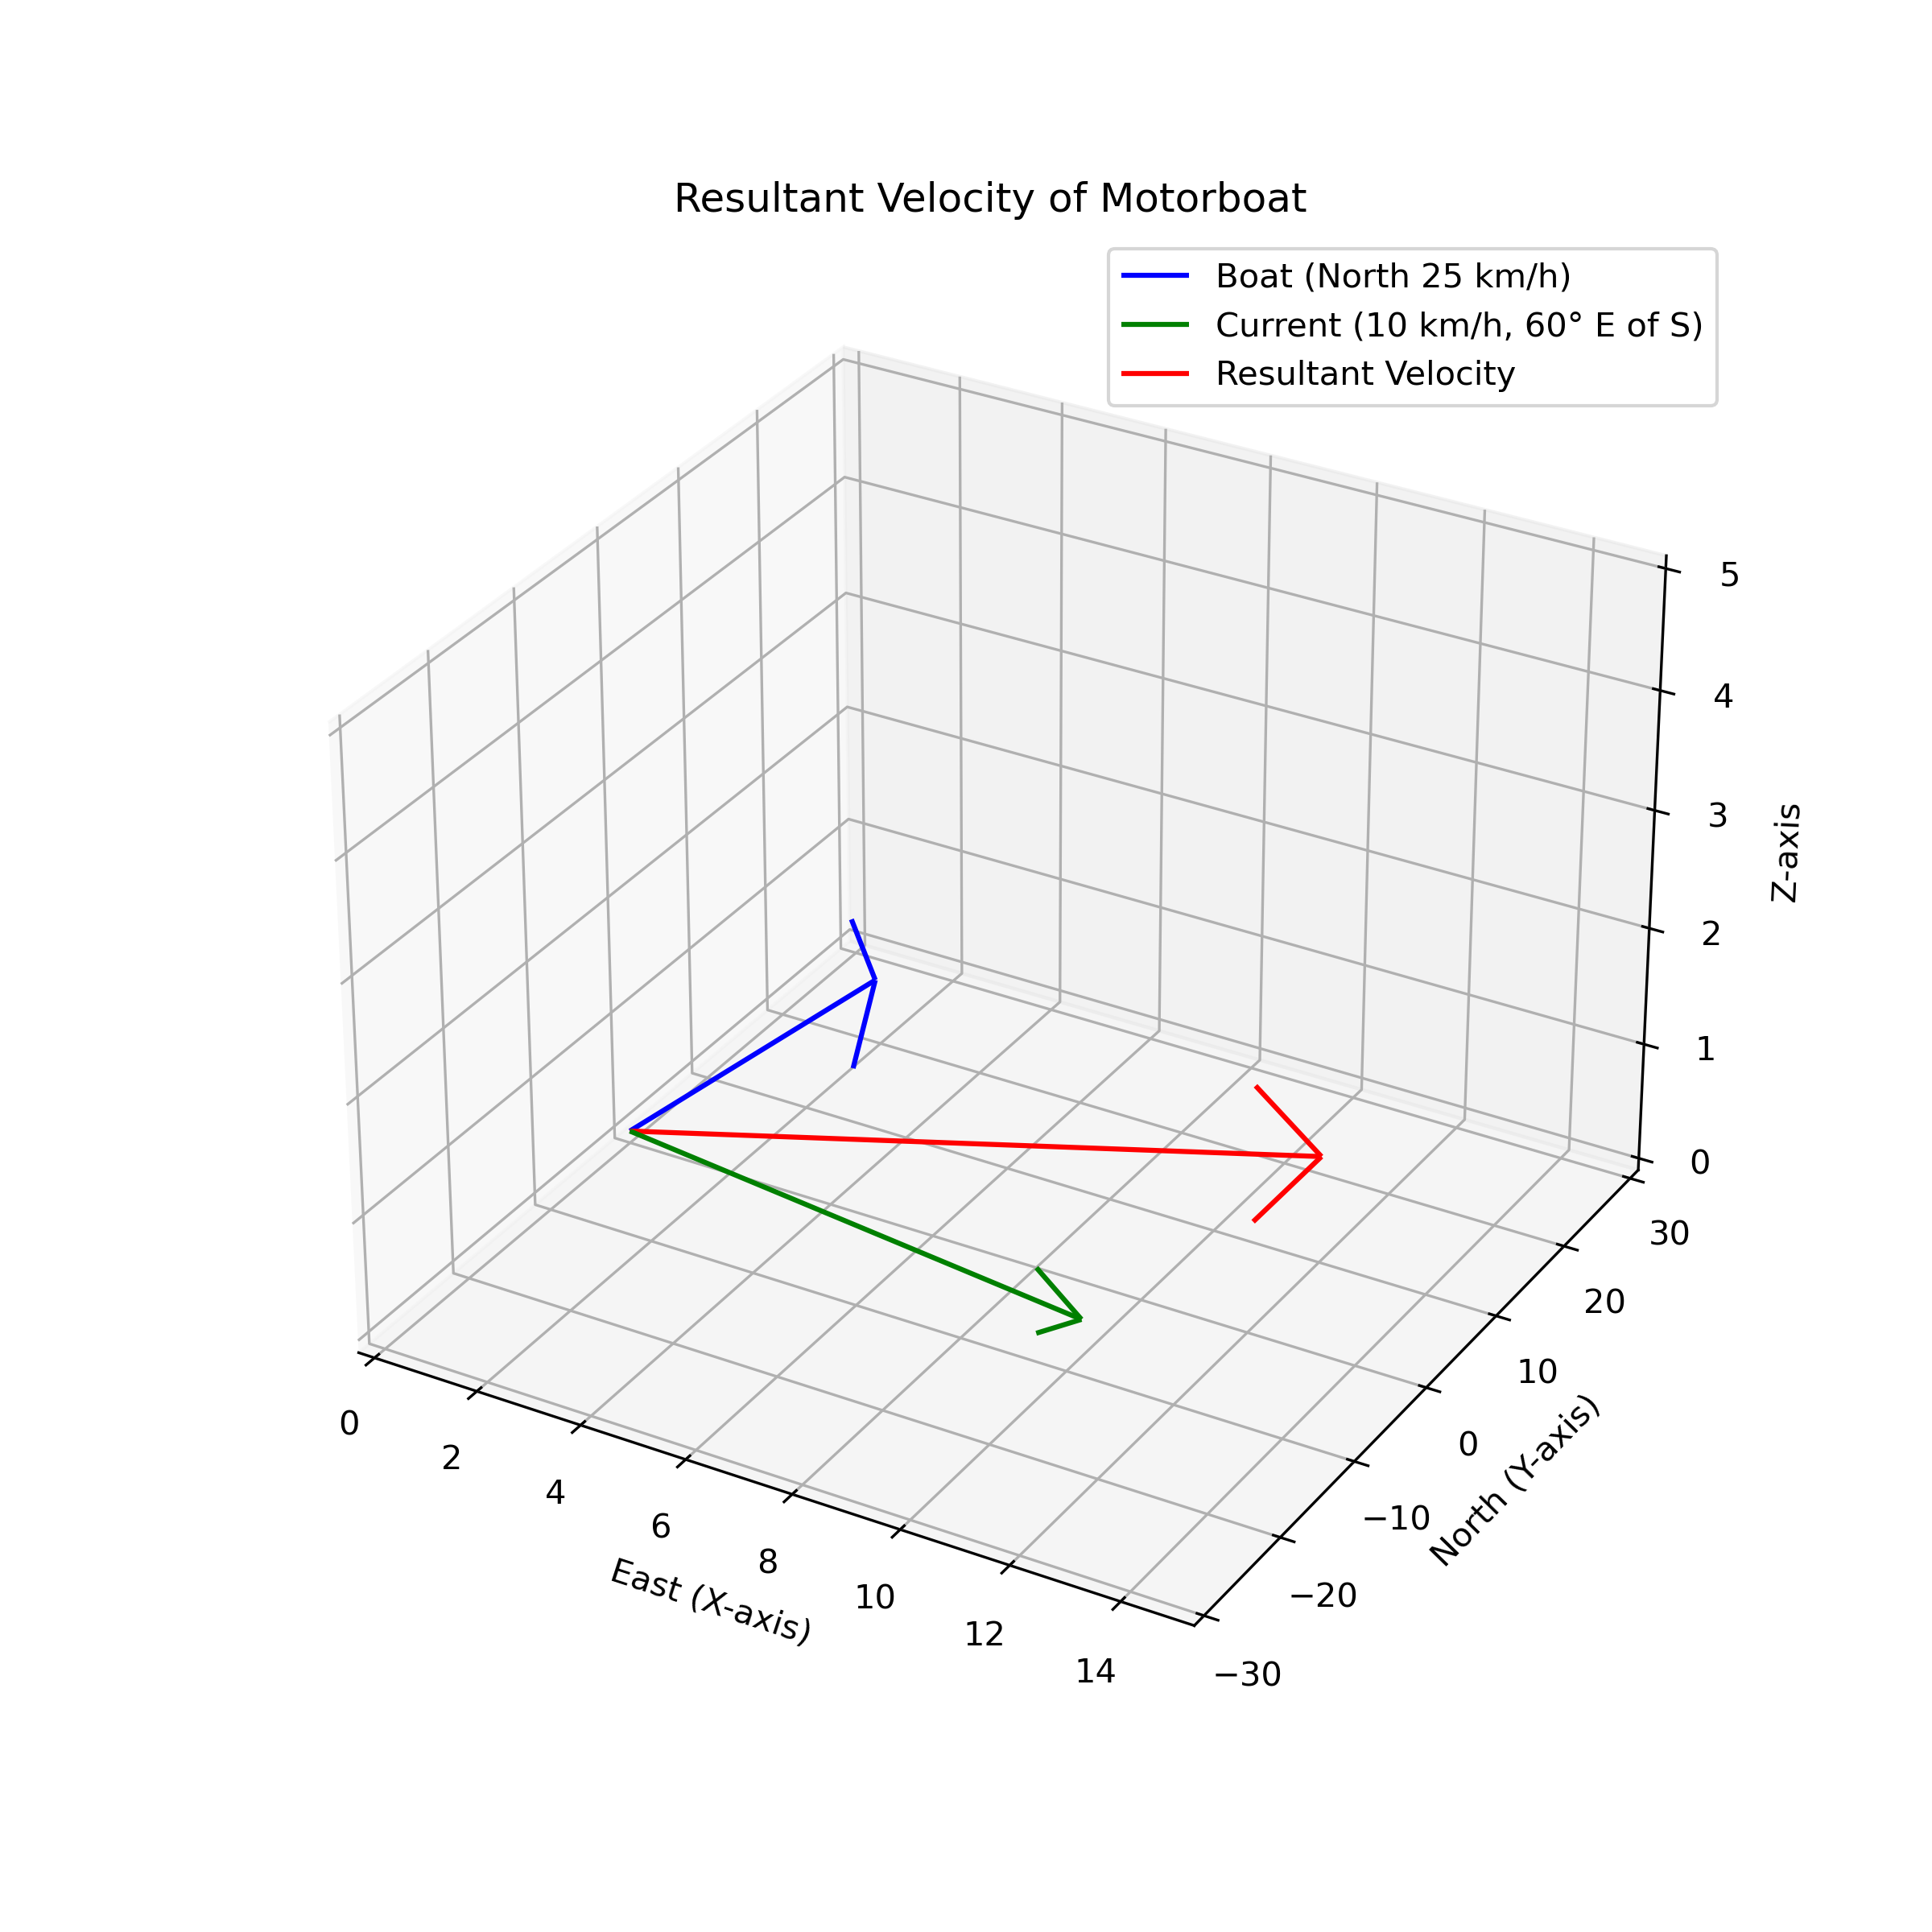
\includegraphics[height=0.5\textheight, keepaspectratio]{figs/fig.png}
    \label{figure_1}
\end{figure}
 


\end{document}